

%%%% Better Poster latex template example v1.0 (2019/04/04)
%%%% GNU General Public License v3.0
%%%% Rafael Bailo
%%%% https://github.com/rafaelbailo/betterposter-latex-template
%%%% 
%%%% Original design from Mike Morrison
%%%% https://twitter.com/mikemorrison
% https://www.agu.org/Ocean-Sciences-Meeting/Pages/Presenter-Guidelines
%\documentclass[a0paper,fleqn]{betterposter}
\documentclass[fleqn]{betterposter}

%%%% Uncomment the following commands to customise the format
%% Setting the width of columns
% Left column
%\setlength{\leftbarwidth}{0.25\paperwidth}
% Right column
%\setlength{\rightbarwidth}{0.25\paperwidth}
%% Setting the column margins
% Horizontal margin
%\setlength{\columnmarginvertical}{0.05\paperheight}
% Vertical margin
%\setlength{\columnmarginhorizontal}{0.05\paperheight}
% Horizontal margin for the main column
%\setlength{\maincolumnmarginvertical}{0.15\paperheight}
% Vertical margin for the main column
%\setlength{\maincolumnmarginhorizontal}{0.15\paperheight}
%% Changing font sizes
% Text font
%\renewcommand{\fontsizestandard}{\fontsize{28}{35} \selectfont}
% Main column font
\renewcommand{\fontsizemain}{\fontsize{108.00}{125.00} \selectfont}

% Title font
\renewcommand{\fontsizetitle}{\fontsize{60}{100} \selectfont}

% Author font
%\renewcommand{\fontsizeauthor}{\fontsize{28}{35} \selectfont}
% Section font
%\renewcommand{\fontsizesection}{\fontsize{28}{35} \selectfont}
%% Changing font sizes for a specific text segment
% Place the text inside brackets:
% {\fontsize{28}{35} \selectfont Your text goes here}
%% Changing colours
% Background of side columns
%\renewcommand{\columnbackgroundcolor}{black}
% Font of side columns
%\renewcommand{\columnfontcolor}{gray}
% Background of main column
\renewcommand{\maincolumnbackgroundcolor}{miamiblue}

%\renewcommand{\maincolumnbackgroundcolor}{theory}
%\renewcommand{\maincolumnbackgroundcolor}{methods}
%\renewcommand{\maincolumnbackgroundcolor}{intervention}
% Font of main column
%\renewcommand{\maincolumnfontcolor}{gray}
\renewcommand{\Pr}[1]{\ensuremath{\operatorname{\mathbb{P}}\!{\left(#1\right)}}} 
\newcommand{\Ex}[1]{\ensuremath{\operatorname{\mathbb{E}}\!{\left(#1\right)}}}

%\graphicspath{{"2020. OSM/figures/"}}
\graphicspath{{"figures/"}}

\begin{document} \betterposter{
%%%%%%%% MAIN COLUMN
\maincolumn{

%%%% Main space
Is the \textbf{lower limb} of the AMOC strictly a \textbf{boundary current} ?

\vspace{0.5em} 
r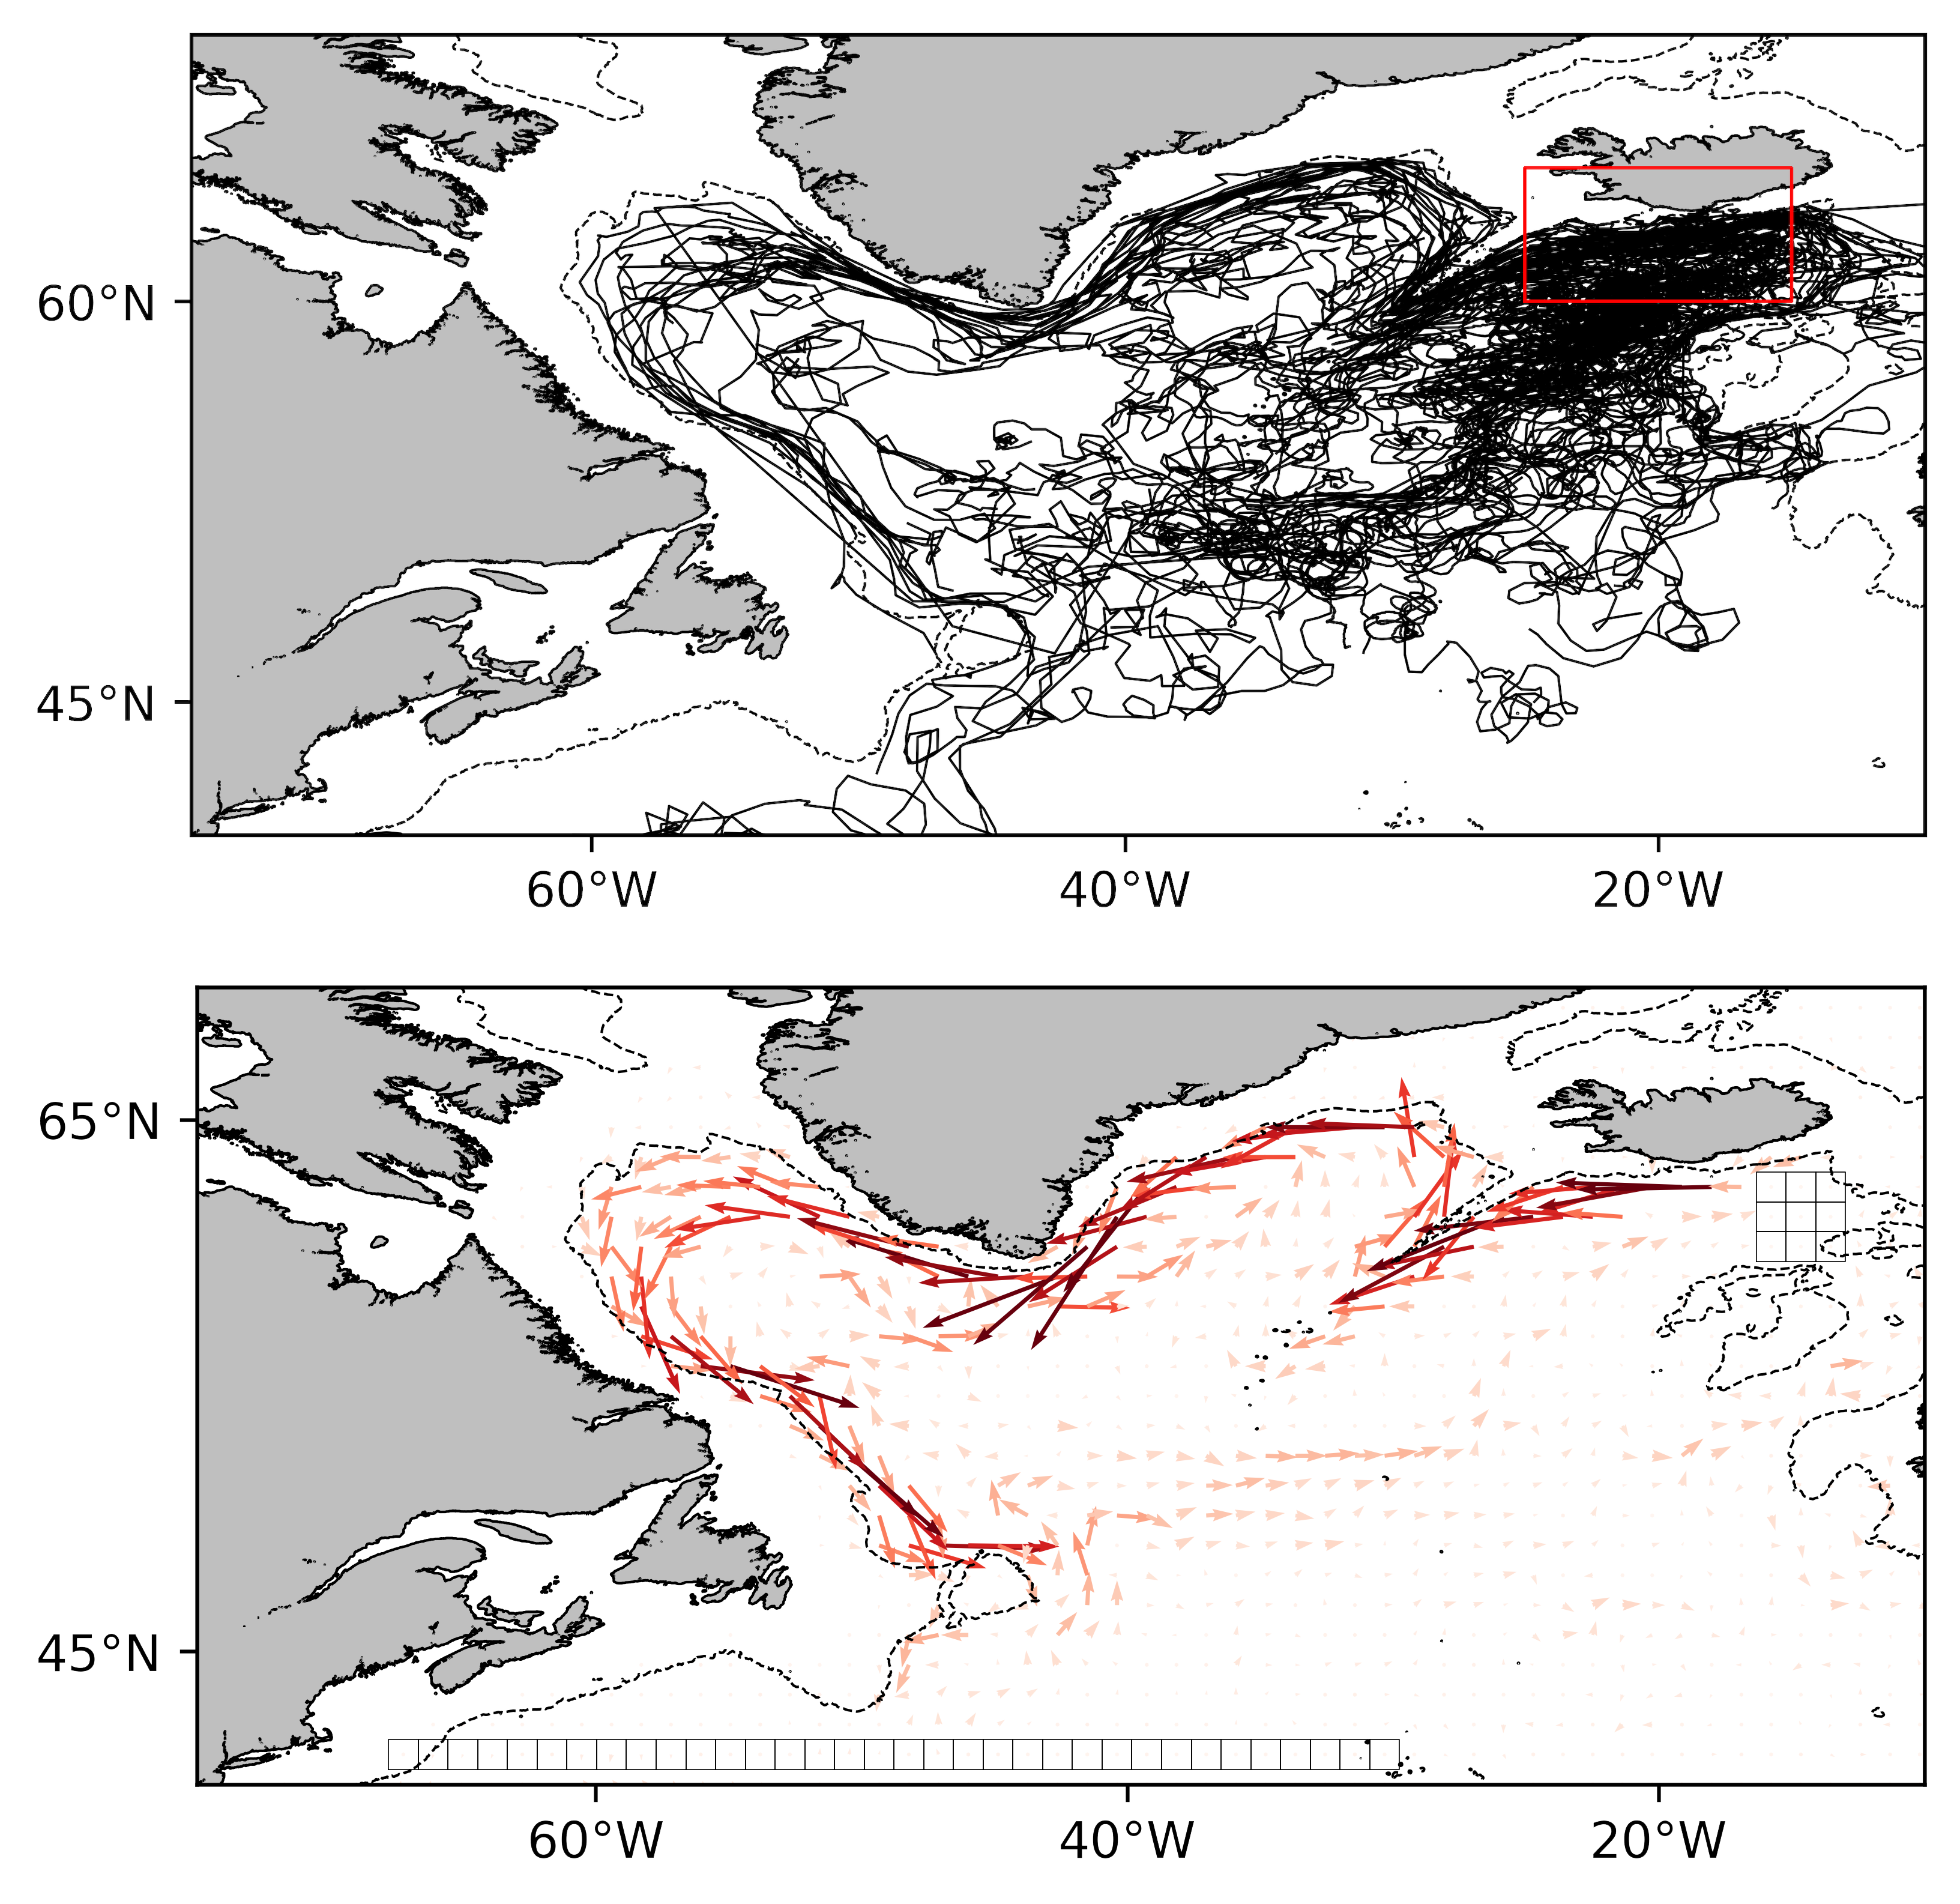
\includegraphics[width=
\textwidth]{na_both.png} 
}{

%%%% Bottom space
%% QR code
% QR code link to papers
\qrcode{figures/qr-code}{figures/smartphone}{ \textbf{Take a picture} to follow \\the project updates. }

% Smartphone icon
% Author: Freepik
% Retrieved from: https://www.flaticon.com/free-icon/smartphone_65680
%% Compact QR code (comment the previous command and uncomment this one to switch)
%\compactqrcode{figures/qr-code}{
%\textbf{Take a picture} to
%\\download the full paper
%}
}

}{

%%%%%%%% LEFT COLUMN
\title{Unveiling North Atlantic Deep Water pathways using nonlinear dynamics techniques} 
\author{P. Miron$^1$, F. J. Beron-Vera$^1$, M. J. Olascoaga$^1$, L. Helfmann$^2$, P. Koltai$^2$ and S. Lozier$^3$} \institution{$^1$University of Miami, Miami} \institution{$^2$Freie Universit\"at, Berlin} \institution{$^3$Duke University, Durham} \institution{\faTwitter\,philippemiron}


\section{\color{miamifushia} Introduction} The North Atlantic Deep water equatorward spreads from high latitudes was expected to be largely contained along the Deep Western Boundary Current.

\vspace{0.2em} New observations from moorings and floats instead showed multiple interior pathways. We propose to analyze deep water circulation from historical Lagrangian observations datasets (Argo and RAFOS floats).


\section{\color{miamifushia} Markov Chain} The information contains in the float trajectories is combined into a transition matrix $P$ representing a Markov Chain of the underlying dynamics. The domain is subdivided into boxes and the entries of $P$ are equal to the conditional transition probabilities between them. 
\begin{equation*}
	P_{ij} = \Pr{x_{t+T}\in B_j \mid x_{t}\in B_i} 
\end{equation*}

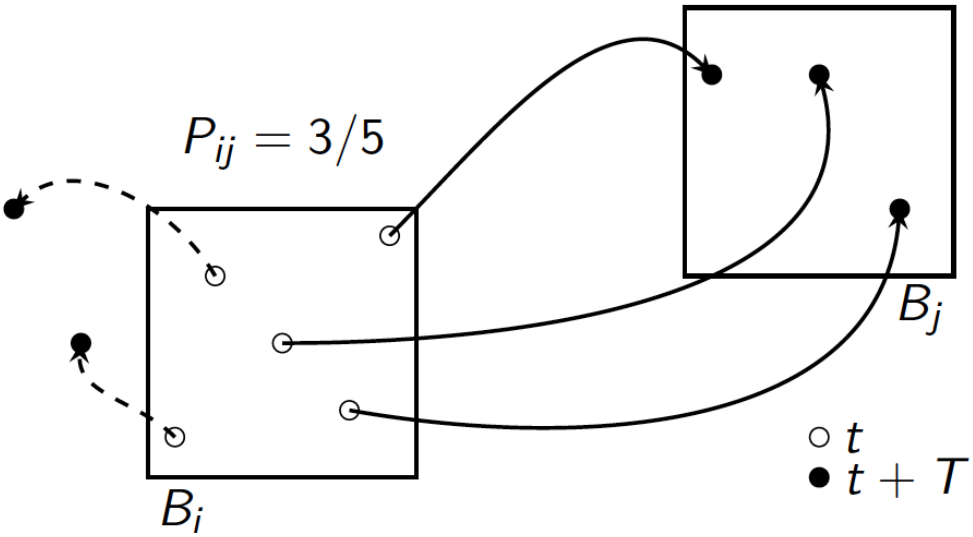
\includegraphics[width=0.9
\textwidth]{pij.png}

%% This fills the space between the content and the logo
%% Institution logo
\vfill 

\includegraphics[width=
\textwidth]{official-um-rsmas.jpg} }{

%%%%%%%% RIGHT COLUMN


\section{\color{miamifushia} Transition Path Theory} From the constructed Markov Chain on the space $\mathbb{S}$, we are interested in the connection between $A$ and $B$, two subsets of the space $\mathbb{S}$. Using techniques from transition path theory, we can extract how this transition takes place, where trajectories spend more time and what are the main channels. Below in red are the reactive trajectories, segments that connect directly sets $A$ to $B$.

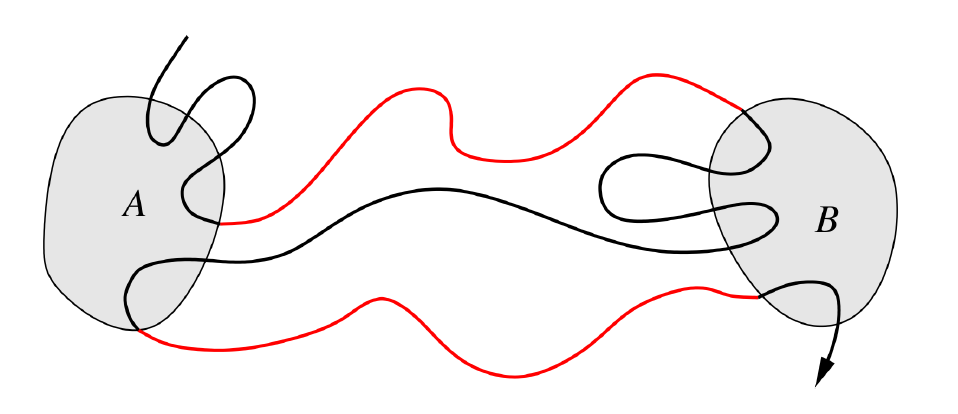
\includegraphics[width=
\textwidth]{reactive-traj.png}


\section{\color{miamifushia} Future work} From surface drifters, deep floats and model outputs, we will investigate the different limbs of the AMOC to characterize the connections between the North Atlantic, where deep water masses are formed, and their sources in the South Atlantic.


\section{\color{miamifushia} References} N. Djurdjevac, Methods for analyzing complex networks using random walker approaches

\vspace{0.15em} L. Helfmann and P. Koltai, Transition path theory for time-dependent dynamics (preprint)

\vspace{0.15em} M. S. Lozier et al., A sea change in our view of overturning in the subpolar North Atlantic

\vspace{0.15em} P. Metzner, Transition path theory for Markov processes

\vspace{0.15em} E. Weinan and E. Vanden-Eijnden, Towards a theory of transition paths. Journal of statistical physics

%% This fills the space
\vfill

%NSF Proposal 1851097
\begin{center}
	
\includegraphics[scale=0.15]{nsf_logo.png} 
\end{center}
} 
\end{document}
